\section{Binary Color Functions}
\label{sec:binary}

While group and segment terms model the dependency of color assignments on features of same-color regions, they do not capture relationships between different-color regions. In particular, adjacent color regions can have strong effects on their neighbor's perceived color, making colors seem more or less saturated or causing vibrating boundaries if adjacent lightness and colorfulness are too similar~\cite{AlbersInteractionOfColor}. Thus, we also predict distributions over color properties for adjacent segment pairs.

\subsection{Color Properties and Predictive Features}
\label{sec:binaryPropsAndFeatures}

As with individual pattern regions, there are many possible properties of the color relationship between two adjacent regions that could influence the appearance of a pattern coloring. Our method uses the following set:
%%%
%\begin{description}[leftmargin=*]
\begin{description}
	\item[Perceptual Difference] is the Euclidean distance between two colors in \lab space and is the primary descriptor of `contrast' between two colors that we use in our model. This distance is a simple and efficient-to-evaluate approximation to perceptual distance; more sophisticated formulae have also been proposed~\cite{CIEDE2000}.
	\item[Relative Lightness] is the absolute difference between the L values of two colors in \lab space. This `difference of intensities' captures another important type of contrast between two colors.
	\item[Relative Colorfulness] is the absolute difference between the colorfulness values of two two colors, using the definition of colorfulness from Section~\ref{sec:unary}. This property helps capture whether or not two colors should be mutually saturated/desaturated
	\item[Chroma Difference] measures the squared fraction of perceptual distance due to the \lab chroma channels: $\frac{\delta a^2+\delta b^2}{\delta a^2+\delta b^2+\delta L^2}$. This value can be interpreted as a more perceptually-grounded version of the `hue angle' between two colors on a color wheel.
	\item[Color Name Similarity] is the cosine similarity between the color name count vectors defined in Section~\ref{sec:unary}~\cite{ColorNamingModels}. This measure assesses whether two colors are typically referred to with the same names.
\end{description}
%%%
To form a set of predictive features for an adjacent segment pair, we use the features from both of the participating segments, concatenating them so that the one with the smaller $L_2$ norm is first to enforce a consistent ordering. We then append an additional pair of features based on the insight that good color assignments to adjacent segments may depend on the nature of their adjacency. For example, a square enclosed by a thin border appears different from a square enclosed by a thick border, and different again from a square side-by-side with another square (Figure~\ref{fig:surround}). Thus, we add a pair of features we call \textbf{Enclosure strengths}, which measure how much one segment in the adjacency encloses the other and vice versa. Enclosure strength is defined as the number of pixels of the neighboring segment appearing within a 2-pixel neighborhood outside the segment's boundary, normalized by the area of that neighborhood. Out-of-image pixels are counted as part of the neighborhood area.

\begin{figure}[ht]
\centering

\includegraphics[width=.7\columnwidth]{figs/surround}
\caption{Color appearance depends on relationships with surrounding regions.}
\label{fig:surround}
\end{figure}

\subsection{Color Property Distributions}
\label{sec:binaryDistribs}

For a particular pair of adjacent segments $(\segment, \segprime)$ and a color property $\prop$, we can define a function for the distribution over color property values given the features of the adjacency:
%%
\begin{equation*}
\adjInstStats(\colors_\segment, \colors_\segprime) = \ln p( \prop( \colors_\segment, \colors_\segprime ) | \features_{\segment, \segprime} ) \cdot \adjStrength(\segment, \segprime)
\end{equation*}
%%
where $\adjStrength(\segment,\segprime)$ is the \emph{strength} of the adjacency $(\segment,\segprime)$. We define adjacency strength as the number of pixels from segments $\segment$ or $\segprime$ that are within a 2-pixel distance from their perimeters. All adjacency strengths in a given pattern are normalized to sum to 1. We learn the distributions $p$ using the `histogram regression' approach described in Section~\ref{sec:unary}.

Figure~\ref{fig:binaryHistograms} shows predicted distributions over relative lightness for two different adjacent segment pairs; a value of 0 indicates identical lightness values. The two distributions are similar in shape and reflect the intution that no two adjacent segments should be completely equi-luminant. However, the foreground-background adjacency between the kite and the sky concentrates more of its mass toward higher lightness differences. Together, these two distributions suggest that foreground-background adjacencies should have higher lightness contrast than foreground-foreground adjacencies.

\begin{figure}[ht]
\begin{tabular}{cc}
{\raisebox{4em}{
\includegraphics[width=.25\columnwidth]{figs/histograms/foregroundAdjacency}}}&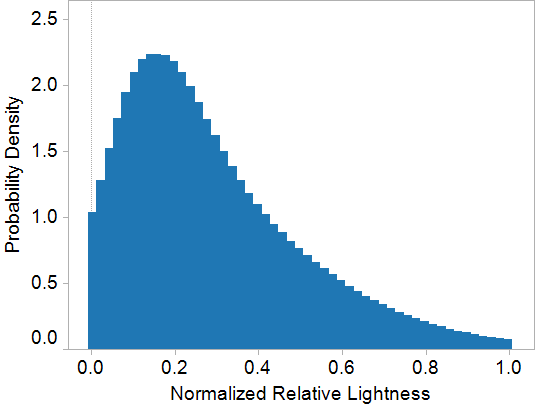
\includegraphics[width=.60\columnwidth]{figs/histograms/foregroundAdjacencyHistogram}\vspace{0.5em}\\
{\raisebox{4em}{
\includegraphics[width=.25\columnwidth]{figs/histograms/foregroundBackgroundAdjacency}}}&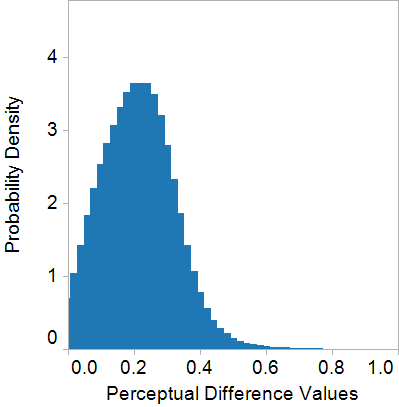
\includegraphics[width=.60\columnwidth]{figs/histograms/foregroundBackgroundAdjacencyHistogram}\vspace{0.5em}\\
\end{tabular}

\caption{Predicted distributions over relative lightness for two different segment adjacencies (participating segments higlighted in orange and green). The foreground-foreground distribution permits more similar lightness values than the foreground-background disribution.}
\label{fig:binaryHistograms}
\vspace{-1.0em}
\end{figure}

%Good color assignments to adjacent segments may depend on the nature of their adjacency. For example, a square enclosed by a thin border appears different from a square enclosed by a thick border, and different again from a square side-by-side with another square (Figure~\ref{fig:surround}). Thus, when computing features of an adjacency we include the features of the segments involved as well as how much one neighbor encloses another.
%\begin{figure}[ht]
%\centering
%
\includegraphics[width=.7\columnwidth]{figs/surround}
%\caption{Color appearance depends on relationships with surrounding regions\remark{Rough figure.}}
%\label{fig:surround}
%\end{figure}
%
%
%Our model has one adjacency term for each of the color properties $ \prop \in \binaryProps$, which are \propName{RelativeLightness}, \propName{RelativeColorfulness}, \propName{PerceptualDifference}, \propName{ChromaDifference}, and \propName{NameSimilarity}.
%As with group and segment terms, \propName{RelativeLightness} and \propName{RelativeColorfulness} are computed in \lab space. \propName{PerceptualDifference} is Euclidean distance in \lab space, and \propName{ChromaDifference} is the percentage of that distance that is due to the chroma channels. Finally, \propName{NameSimilarity} is the color name cosine similarity measure defined by Heer and Stone~\shortcite{ColorNamingModels}.
%
%The sufficient statistics function for each binary property is:
% \begin{align*}
% \adjTerm(\colors | \pattern) &= \sum_{(\segment, \segprime) \in \adj(\pattern)} \adjInstStats(\colors_\segment, \colors_\segprime | \pattern, \segment, \segprime) \\
% \adjInstStats(\colors_\segment, \colors_\segprime | \pattern, \segment, \segprime) &= \ln p( \prop( \colors_\segment, \colors_\segprime ) | \features_{\segment, \segprime} ) \cdot \adjStrength(\segment, \segprime)
%\end{align*}
%where $\adjStrength(\segment,\segprime)$ is the strength of the adjacency $(\segment,\segprime)$. We define adjacency strength as the number of pixels from segments $\segment$ or $\segprime$ that are within a 2-pixel distance from their perimeters. All adjacency strengths are normalized to sum to 1.  
%
%These terms contribute binary factors over each adjacent pair of color variables:
%\begin{equation*}
% \factor(\colorVars_\group, \colorVars_\groupprime | \pattern) = \prod_{\prop \in \binaryProps} \exp( (\adjTermWeight \cdot \sum_{\mathclap{(\segment, \segprime) \in \adj(\group, \groupprime)}} \adjInstStats( \colorVars_\group, \colorVars_\groupprime | \pattern, \segment, \segprime))) 
%\end{equation*}